\documentclass[12pt]{report}

\usepackage{setspace}
%\setstretch{2.5} % for custom spacing
\setlength{\parindent}{4em}

\usepackage{fancyvrb}
\usepackage{graphicx}
\usepackage{geometry}

\geometry{letterpaper, portrait, margin=1in}

%%%Title Page%%%
\title{
  Lab 04
\bigbreak General Sequential Logic Simulation
}

\author{
{\normalsize
\begin{tabular}{l r r}
 & \textbf{Ryan Cruz} & \textbf{Zachary Davis}\\
\textbf{Category} & ryan.cruz25@uga.edu & zachdav@uga.edu\\
\hline
Pre-lab & NA & NA\\
In-lab Module \& Testbench Design & 50 & 50\\
In-lab Testbench Sim. \& Analysis & 50 & 50\\
In-lab FPGA Synthesis \& Analysis & NA & NA\\
Lab Report Writing & 50 & 50\\
\end{tabular}
}
}

\date{\bigskip
October 5, 2017}
%%%%%%%%%%%%


\begin{document}
\maketitle

\section*{Lab Purpose}
	\paragraph{}
	In this lab we practice designing basic sequential logics and use a Finite State Machine (FSM) to capture and design simple sequential circuits in Verilog. There is no physical 
	FPGA implementation for this lab.  The focus of the lab is on writing code and simulation rather than implementation.

\section*{Implementation Details}
	\subsection*{Pre-Lab Reading}
		\paragraph{}
		There was no pre-lab to turn in for this lab, just reading from text to be prepared for lab.
	\subsection*{8-Bit Register}
		\textbf{Behavioral Module Code}
		\begin{Verbatim}[frame=single, fontsize=\small]
`timescale 1ns / 1ps
////////////////////////////////////////////////////////////////////////////////
// Engineer: Zachary Davis & Ryan Cruz
// 
// Create Date:    16:37:09 10/02/2017 
// Design Name:     Eight_Bit_Register
// Module Name:    Eight_Bit_Register 
//
// Revision: 
// Revision 0.01 - File Created
// Additional Comments: 
//
////////////////////////////////////////////////////////////////////////////////
module Eight_Bit_Register(D, Q, Clk, Reset);

	input Clk, Reset;
	input [7:0] D;
	output [7:0] Q;
	reg [7:0] Q;
	
	always@(posedge Clk)
	begin
	
		if (Reset == 1)
			Q <= 0;
		else
			Q <= D;

	end
endmodule

		\end{Verbatim}
		
		\flushleft
		\textbf{Test Bench Code}
		\begin{Verbatim}[frame=single, fontsize=\small]
`timescale 1ns / 1ps
////////////////////////////////////////////////////////////////////////////////
// Engineer: Zachary Davis & Ryan Cruz
// 
// Create Date:    18:05:49 10/02/2017 
// Design Name:     Eight_Bit_Register_Test_Bench
// Module Name:    Eight_Bit_Register_tb 
//
// Revision: 
// Revision 0.01 - File Created
// Additional Comments: 
//
////////////////////////////////////////////////////////////////////////////////
module Eight_Bit_Register_tb();

	reg Clk_t, Reset_t;
	reg [7:0] D_t;
	wire [7:0] Q_t;

	Eight_Bit_Register Eight_Bit_Register_1(D_t, Q_t, Clk_t, Reset_t);

	always 
	begin
	
		Clk_t <= 0; 
		#10;  
		Clk_t <= 1; 
		#10; 

	end 
	
	initial
	begin
		
		Reset_t <= 1; 
		D_t <= 255;

		@(posedge Clk_t)
		#5 Reset_t <= 0; 
		D_t <= 1;
		
		@(posedge Clk_t)
		#5 Reset_t <= 0; 
		D_t <= 2;
		
		@(posedge Clk_t)
		#5 Reset_t <= 1; 
		D_t <= 140;
		
		@(posedge Clk_t)
		#5 Reset_t <= 0; 
		D_t <= 69;
		
		@(posedge Clk_t)
		#5 Reset_t <= 0; 
		D_t <= 240;
		
		@(posedge Clk_t)
		#5 Reset_t <= 0; 
		D_t <= 97;
		
		@(posedge Clk_t)
		#5 Reset_t <= 0; 
		D_t <= 78;
		
		@(posedge Clk_t)
		#5 Reset_t <= 1; 
		D_t <= 136;
		
		@(posedge Clk_t)
		#5 Reset_t <= 0; 
		D_t <= 97;
		
		@(posedge Clk_t)
		#5 Reset_t <= 0; 
		D_t <= 21;
		
		@(posedge Clk_t)
		#5 Reset_t <= 0; 
		D_t <= 36;
		
	end
endmodule
		\end{Verbatim}
		
	\subsection*{4-High-Cycle Laser}
		\textbf{Behavioral Module Code}
		\begin{Verbatim}[frame=single, fontsize=\small]
`timescale 1ns / 1ps
////////////////////////////////////////////////////////////////////////////////
// Engineer: Zachary Davis & Ryan Cruz
// 
// Create Date:    15:46:24 09/29/2017 
// Design Name: 	 4 Cycle High Laser
// Module Name:    Cycle_Laser 
// Project Name: 	 4 Cycle High Laser
// Description: 	 The simulates a laser turning on after a button
//						 press for four cycles.
//
// Revision: 
// Revision 0.01 - File Created
// Additional Comments: 
//
////////////////////////////////////////////////////////////////////////////////
module Cycle_Laser(B, X, Clk, Reset);
	input B, Clk, Reset;
	output X;
	reg X;
	reg [2:0] State, State_Next;
	
	parameter
		S_Off = 0,
		S_On1 = 1,
		S_On2 = 2,
		S_On3 = 3,
		S_On4 = 4;
		
	always@(posedge Clk)
	begin
		if(Reset == 1)
			State <= S_Off;
		else
			State <= State_Next;
	end	
	
	always@(State, B)
	begin
		case(State)
			S_Off:
			begin
				X <= 0;
				if (B == 0)
					State_Next <= S_Off;
				else
					State_Next <= S_On1;
			end
			
			S_On1:
			begin
				X <= 1;
				State_Next <= S_On2;
			end
			
			S_On2:
			begin
				X <= 1;
				State_Next <= S_On3;
			end
			
			S_On3:
			begin
				X <= 1;
				State_Next <= S_On4;
			end
			
			S_On4:
			begin
				X <= 1;
				State_Next <= S_Off;
			end
		endcase
	end
	endmodule
		\end{Verbatim}

		\textbf{Test Bench Code}
		\begin{Verbatim}[frame=single, fontsize=\small]
`timescale 1ns / 1ps
////////////////////////////////////////////////////////////////////////////////
// Engineer: Zachary Davis & Ryan Cruz
// 
// Create Date:    15:46:24 09/29/2017 
// Design Name: 	 4 Cycle High Laser
// Module Name:    Cycle_Laser_tb
// Project Name: 	 4 Cycle High Laser
// Description: 	 The simulates a laser turning on after a button
//						 press for four cycles.
//
// Revision: 
// Revision 0.01 - File Created
// Additional Comments: 
//
////////////////////////////////////////////////////////////////////////////////
module Cycle_Laser_tb();
	reg B_t, Clk_t, Reset_t;
	wire X_t;
	
	Cycle_Laser Cycle_Laser_1(B_t, X_t, Clk_t, Reset_t);
	
	always
	begin
		Clk_t <= 0;
		#10;
		Clk_t <= 1;
		#10;
	end
	
	initial
	begin
		Reset_t <= 1;
		B_t <= 0;
		
		@(posedge Clk_t);
		#5 Reset_t <=0;
		@(posedge Clk_t);
		#5 B_t <= 1;
		@(posedge Clk_t);
		#5 B_t <= 0;
		@(posedge Clk_t);
		@(posedge Clk_t);
		@(posedge Clk_t);
		@(posedge Clk_t);
		#5 B_t <= 1;
		@(posedge Clk_t);
		#5 B_t <= 0;
		@(posedge Clk_t);
		#5 B_t <= 1;
		@(posedge Clk_t);
		#5 B_t <= 0;
		#5 Reset_t <= 1;
	end
endmodule
		\end{Verbatim}
		\vspace{4cm}

	
\section*{Experimental Results}
	
	\subsection*{8-Bit Register}
		\begin{center}
			\textbf{Waveform From 0ns --- 100ns}
			\includegraphics[scale=.47]{tb_1.PNG}
		\end{center}
		\begin{center}
			\textbf{Waveform From 100ns --- 200ns}
			\includegraphics[scale=.47]{tb_2.PNG}
		\end{center}
		\begin{center}
			\vspace {7cm}
			\textbf{Waveform From 200ns --- 300ns}
			\includegraphics[scale=.47]{tb_3.PNG}
		\end{center}
		
		\paragraph{}
		The waveform of Eight\_Bit\_Register acts exactly how a syncronous reset 8-Bit register should.  If the value of the clock and the reset switch are both 1, then 
		the output value is 0 on all eight output pins or 0 in binary.  Otherwise if the value of the reset switch is 0, then D, the ouput, will reflect the value of Q, the input, 
		on the next rising clock edge.  Note that the value of Q before the first rising clock edge is undefined.

	\subsection*{4-High-Cycle Laser}
		\begin{center}
			\textbf{Waveform Result}
			\includegraphics[scale=.59]{tb.PNG}
		\end{center}		

		\paragraph{}
		This waveform acts as a 4 High Cycle laser should.  When the button is pressed, or 1, on the next clock cycle the laser, or X, will go high for 4 clock
		cycles, or four states.  If the button is pressed while the laser is already on we do not want this affect the state of the laser by reseting it or extending the
		number of on states.  This can be seen the second time the button is pressed successfully in the waveform.  Notice that after the laser is activated a second
		time it does nothing to the output X, as it should.  However, the second time the laser is activated it does end after just three clock cycles.  This is not
		because of another button press but instead because on the fourth clock cycle the reset switch has a high value, which returns the laser to the looping
		off state in the FSM.  Like the register note that the value of X, the output, is undefined until the first rising clock edge.

\section*{Significance}
	\paragraph{}
	This lab helped us practice writing code in Xilinx and implement more complex flow of control.  We learned how to use inputs and outputs like D and Q that have
	seven pins as one more readable variable.  We continued to use conditional code, which we first used a couple of labs previous.  Finally, we were able to start working with
	a clock cycle and the conidtional case statements in Verilog when implementing the 4 cycle laser.
	
\section*{Comments/Suggestions}
	\paragraph{}
	It would probaby be a good idea to make drawing a state register and the laser FSM part of a pre-lab in the future just because of how helpful they are and almost
	necessary to completing this lab most effectively.  It also would have been cool to implement this on the FPGA board were perhaps an LED would blink a number of
	times equal to the number of on states for the laser and testing the button reset switch.  Otherwise, the lab was one of the easiest labs yet, but it was more interesting
	working with some more complex code then we have to date.	

\vspace{8cm}
\section*{Additional Lab Specific Information}
	\paragraph{}
	\begin{center}
		\textbf{8-Bit Register Schematic}
		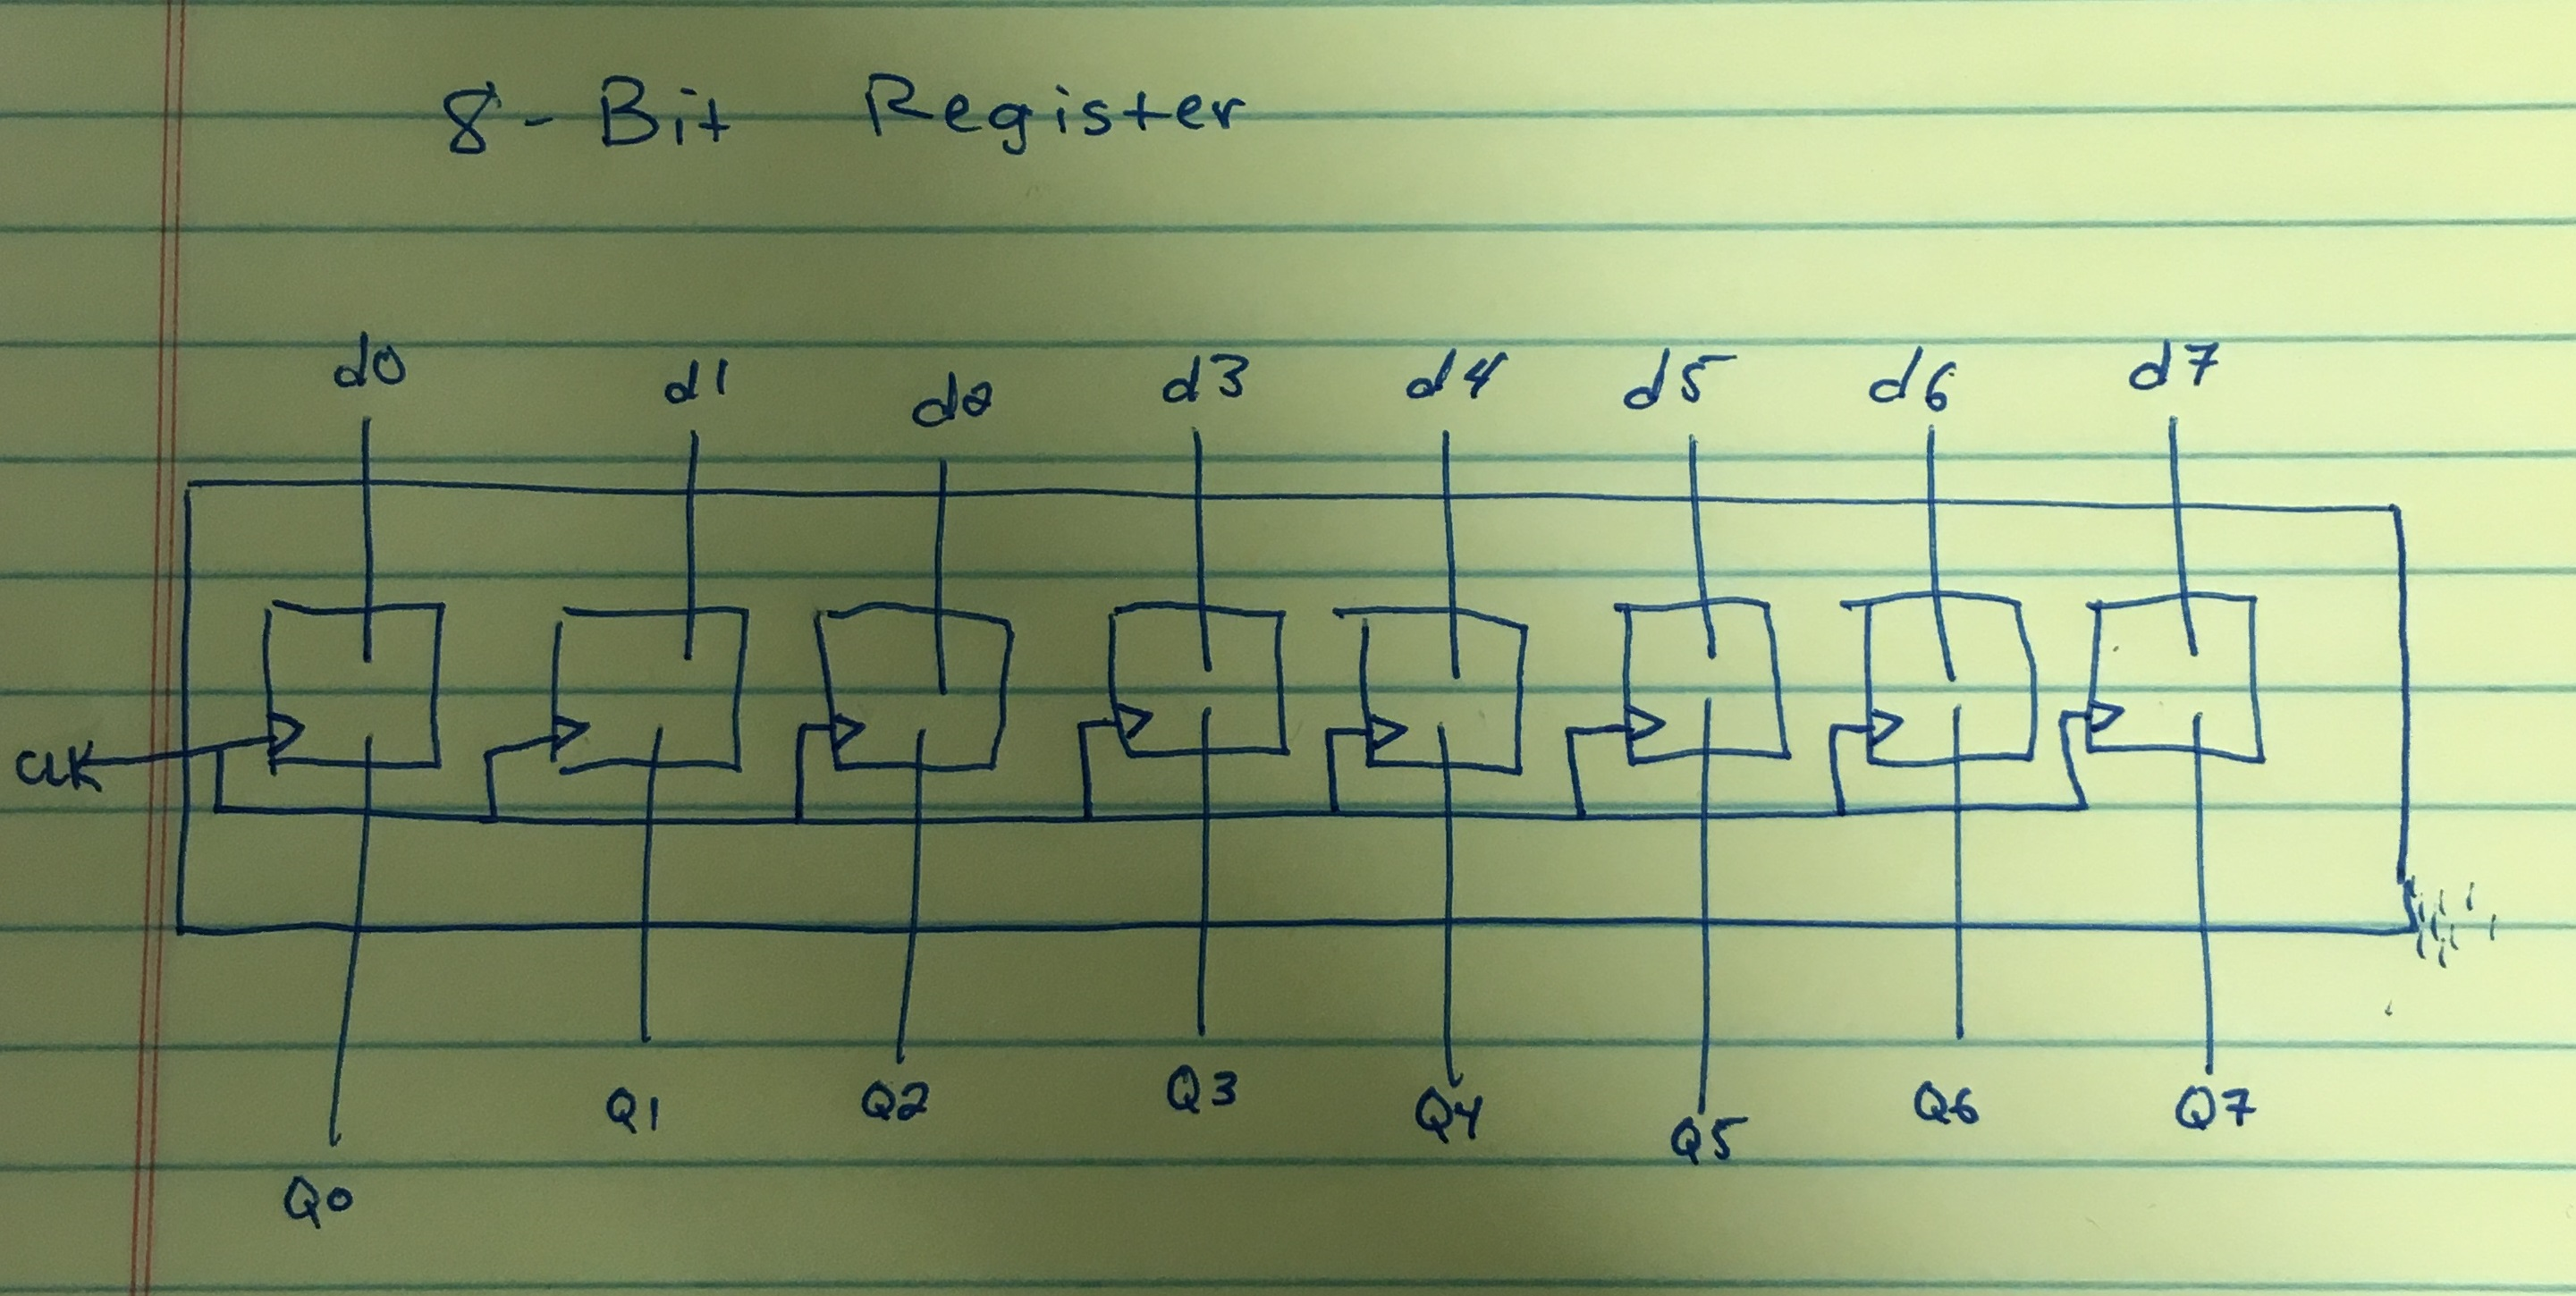
\includegraphics[scale=.15]{register.PNG}
	\end{center}

	\begin{center}
		\textbf{4 Cycle Laser Finite State Machine}
		\includegraphics[scale=.17]{laser.PNG}
	\end{center}

\end{document}